\paragraph{Any size matrix handling}

The following paragraph focuses on the challenge of \textbf{handling matrix multiplication for matrices of arbitrary size} using tiled matrix multiplication. Often, real-world applications require support for matrices that aren't always square or multiples of the tile width (\texttt{TILE\_WIDTH}). So \emph{what is the strategy for these situations?}

\highspace
\begin{flushleft}
    \textcolor{Red2}{\faIcon{exclamation-triangle} \textbf{Limitations of the Tiled Matrix Multiplication presented}}
\end{flushleft}
\begin{itemize}
    \item The base kernel can only handle square matrices whose dimensions are multiples of \texttt{TILE\_WIDTH}. This is a major limitation, since non-square matrices also exist.

    \item A possible solution would be to apply padding, but padding these matrices to match tile sizes can result in \textbf{significant overhead} in terms of space and data transfer time.
\end{itemize}
The basic idea is that instead of padding, a different technique is proposed to efficiently handle matrices of arbitrary size and prevent access to invalid memory locations.

\begin{examplebox}[: graphical example]
    Imagine we have a $3 \times 3$ matrix and a \texttt{TILE\_WIDTH} of 2. The grid and block configuration may result in some threads accessing positions outside the bounds of the $3 \times 3$ matrix.

    The basic logic will be:
    \begin{itemize}
        \item Threads within the valid range of the matrix will load elements normally.
        \item Threads outside the valid range need conditions to avoid accessing or writing to out-of-bound elements.
    \end{itemize}

    Graphically, the special cases that we need to deal with will be:
    \begin{itemize}
        \item When we load elements from the matrix into shared memory:
        \begin{center}
            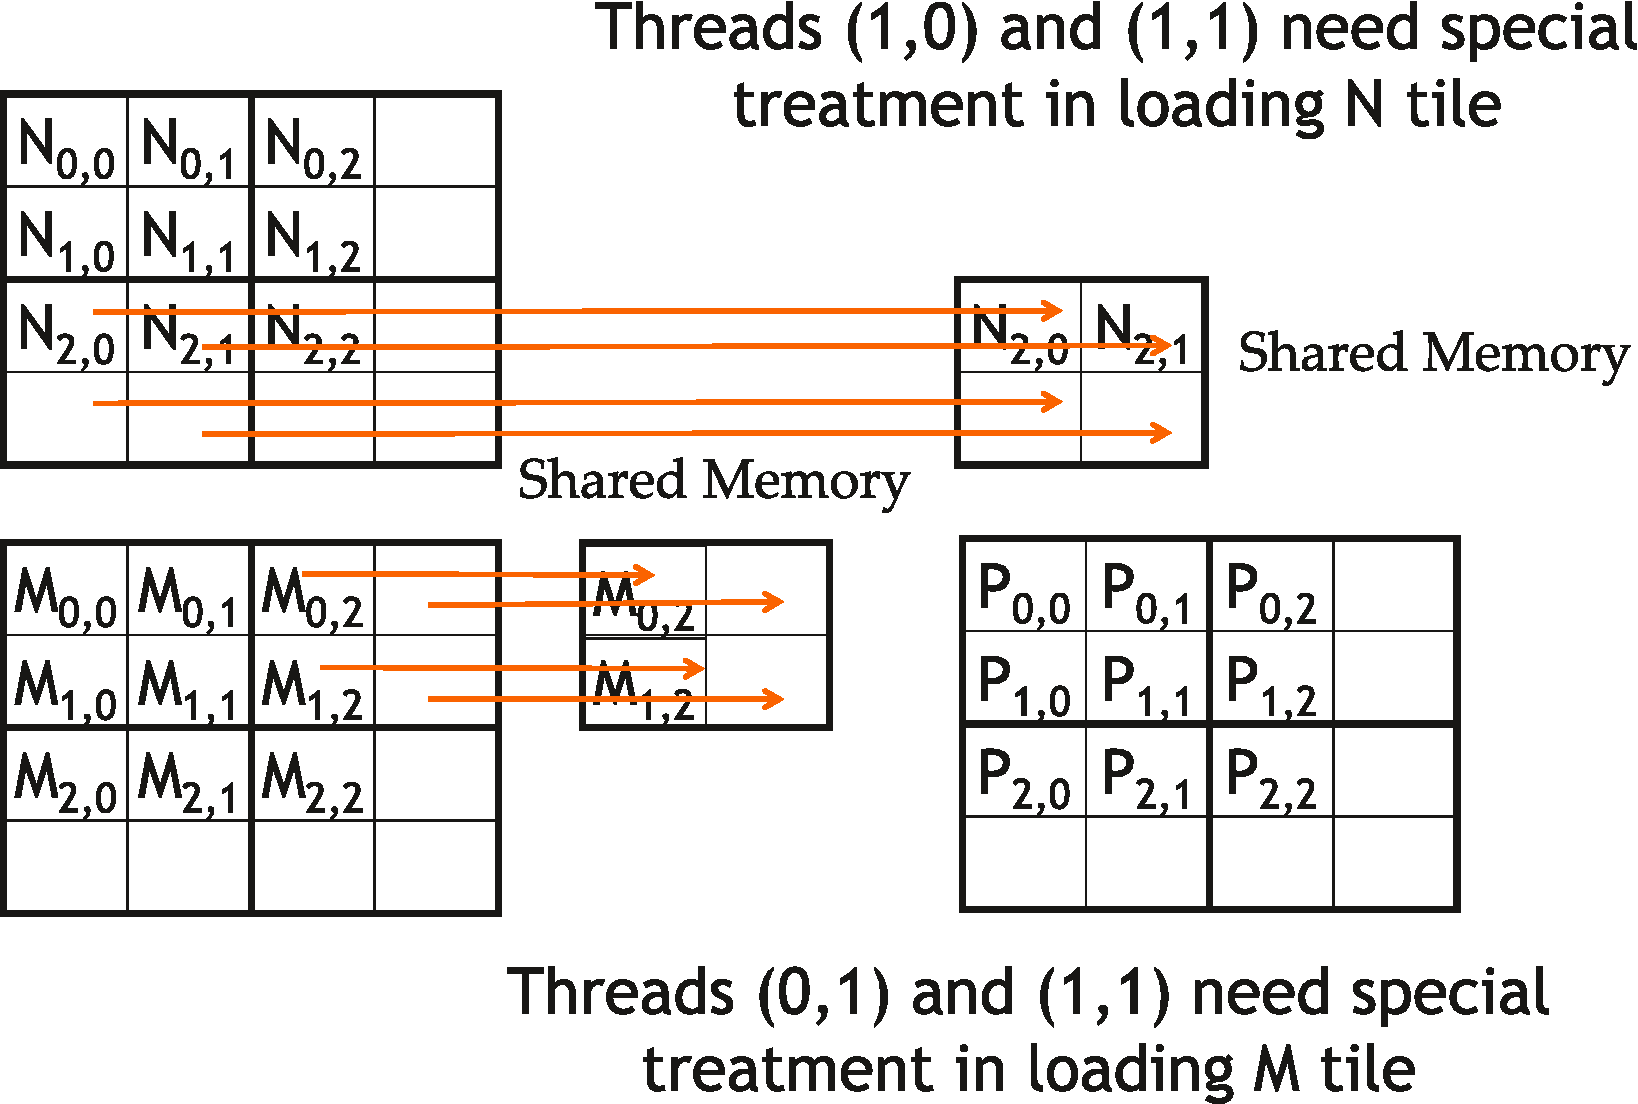
\includegraphics[width=.8\textwidth]{img/cuda-any-size-tile-1.pdf}
        \end{center}
        And:
        \begin{center}
            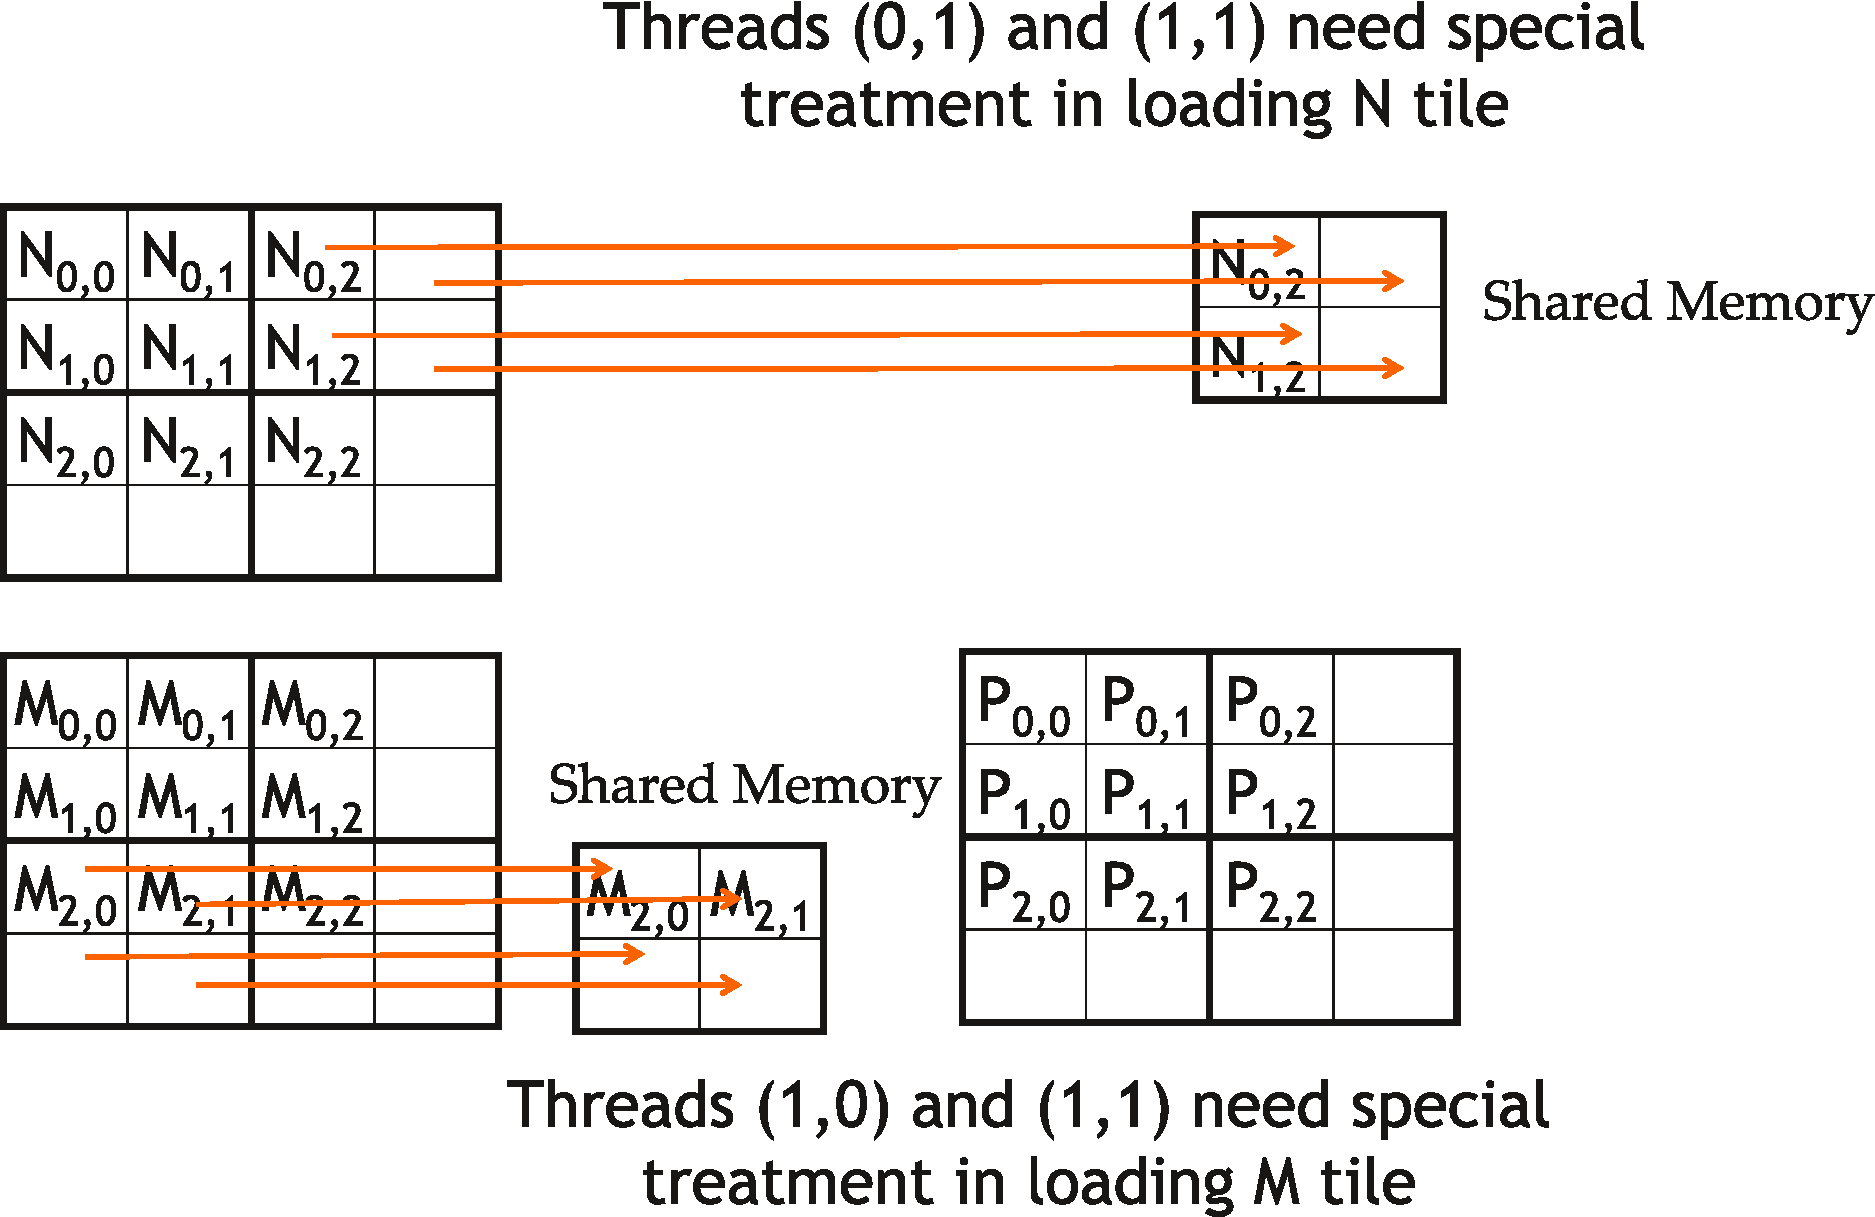
\includegraphics[width=.8\textwidth]{img/cuda-any-size-tile-2.pdf}
        \end{center}

        \item If we use the out-of-bound elements to calculate the result:
        \begin{center}
            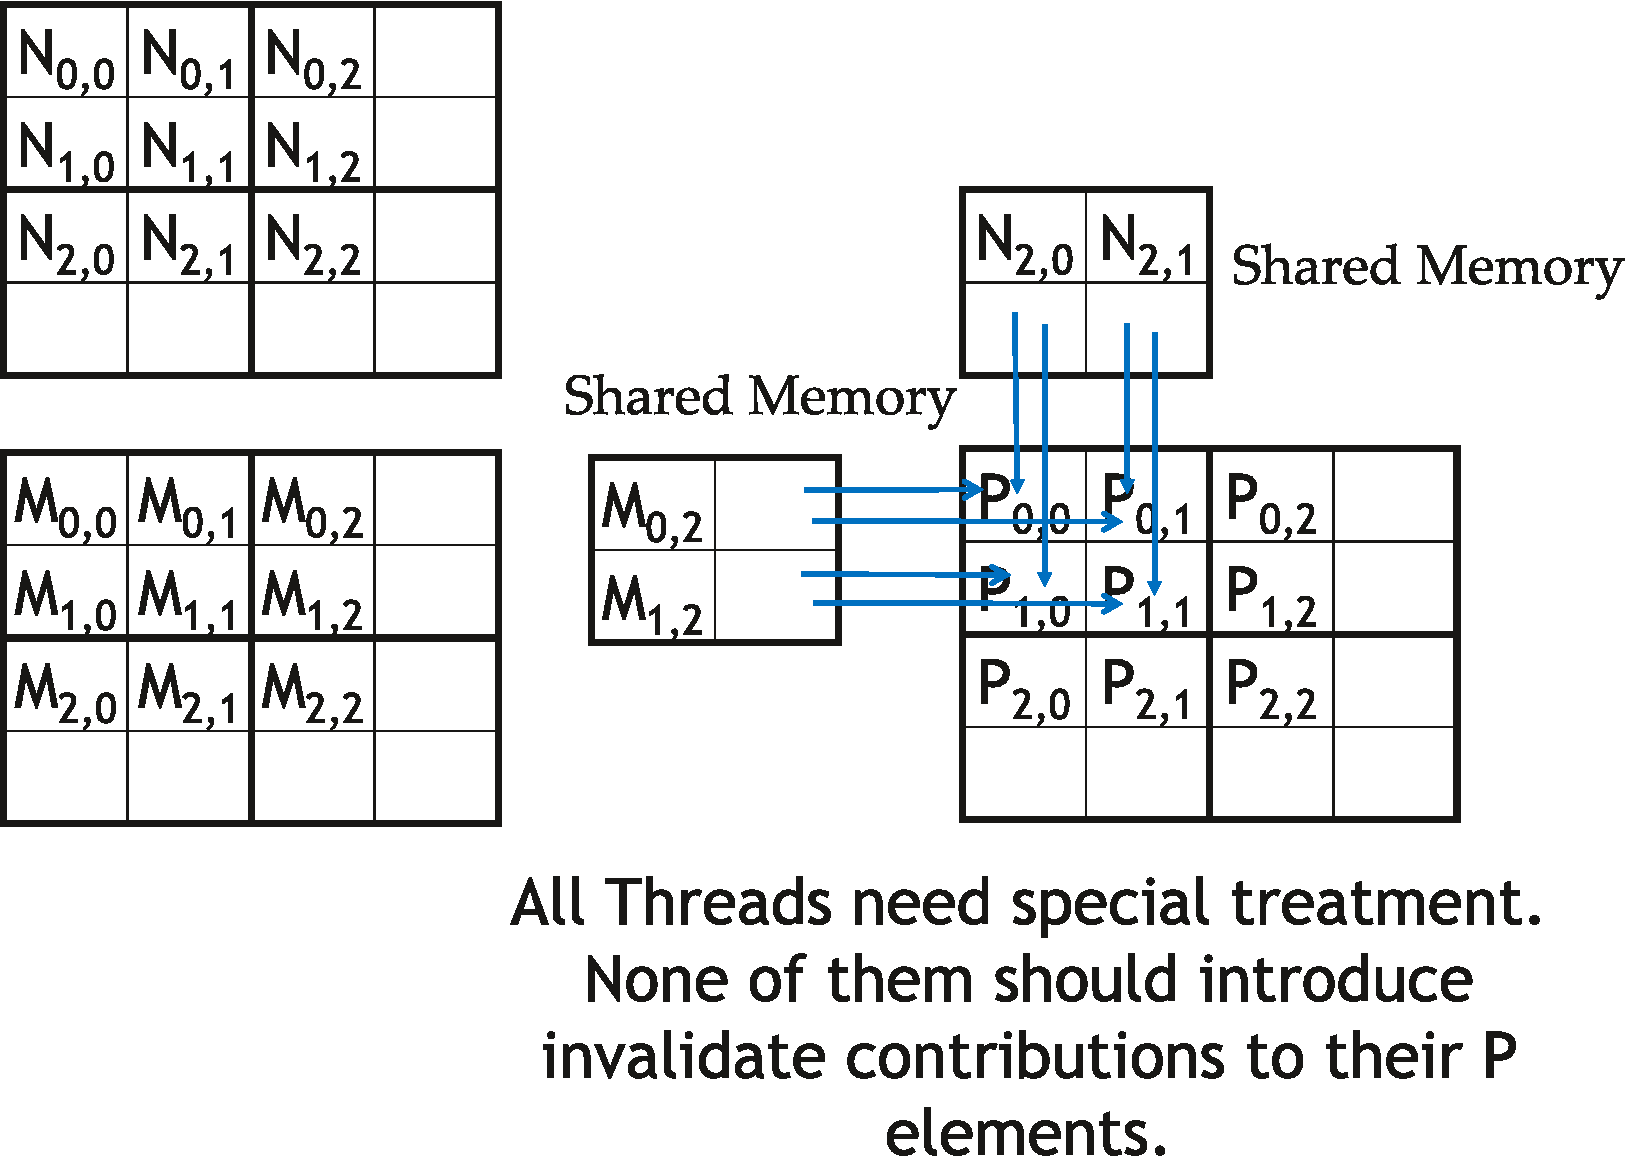
\includegraphics[width=.8\textwidth]{img/cuda-any-size-tile-3.pdf}
        \end{center}
    \end{itemize}
\end{examplebox}

\highspace
\begin{flushleft}
    \textcolor{Green3}{\faIcon{check} \textbf{A simple solution}}
\end{flushleft}
The main simple and efficient solution is the \textbf{conditional loading}. When a thread is to load an input element, \textbf{check if the element index is within valid bounds}:
\begin{itemize}
    \item If \underline{valid}: proceed to \textbf{load the element}.
    \item If \underline{invalid}: do not load the element, but \textbf{write a 0} instead.
\end{itemize}
Assigning a \textbf{0 value ensures that the multiply-add step does not affect the final value of the output element}. Also, this simple check helps \textbf{avoid errors from invalid memory access and ensures correctness}.

\highspace
\begin{flushleft}
    \textcolor{Green3}{\faIcon{question-circle} \textbf{Why do we have to load a zero? We cannot skip this part directly?}}
\end{flushleft}
\begin{enumerate}
    \item \textbf{Safety and Validity}. When a thread loads a 0 instead of an out-of-bound element, it \textbf{ensures that the memory access is valid and does not cause runtime errors or fetch garbage data}. This is crucial for maintaining the stability of the program.

    \item \textbf{Maintaining Computational Integrity}. The 0 value acts as a \textbf{neutral element in multiplication}, meaning it does not alter the final sum during the multiply-add operations. For example:
    \begin{equation*}
        \texttt{
            sum += tileM[ty][k] * tileN[k][tx]
        }
    \end{equation*}
    If \texttt{tileM[ty][k]} or \texttt{tileN[k][tx]} is 0, the sum remains unaffected by that particular operation, preserving the integrity of the calculation.
    
    \item \textbf{Facilitating Parallel Execution}. In CUDA, all threads in a warp (a group of 32 threads) execute the same instruction simultaneously. If some threads are out-of-bound, they still participate in the synchronization and memory access patterns, \textbf{ensuring the warp executes efficiently without branching or divergence}.
    
    By loading 0s, these threads can reach synchronization points (such as \texttt{\_\_syncthreads()}) together with other threads that load valid data, ensuring all threads in the block stay in sync.

    A \definition{Warp Divergence} occurs when \textbf{threads in a warp follow different execution paths due to conditional branches}. This means some threads are active while others are idle, leading to inefficiency. The consequences of warp divergence can have a \textbf{severe impact on performance}.
    \begin{itemize}
        \item \emph{Performance Impact}:
        \begin{itemize}
            \item Divergence causes \textbf{some threads to stall while others execute}, reducing the overall throughput.
            \item \textbf{All threads in the warp must eventually reconverge to execute the same instructions again}, prolonging the execution time for that warp.
        \end{itemize}

        \item \emph{Synchronization Issues}:
        \begin{itemize}
            \item Skipping \texttt{\_\_syncthreads()} or similar synchronization points can lead to incorrect behavior. Threads that do not wait might access incomplete or inconsistent data in shared memory, leading to incorrect results.
            \item \textbf{Ensuring that all threads in a warp (or block) reach synchronization points is crucial for data consistency}.
        \end{itemize}
    \end{itemize}
    
    \item \textbf{Shared Memory Utilization}. All threads, including those loading 0s, contribute to filling the shared memory tiles. This \textbf{ensures that when the matrix multiplication is performed, the shared memory contains a complete tile} (with zeros in out-of-bound areas). This approach guarantees that the shared memory tiles are properly used for the block's calculations, and threads with 0 elements help maintain the structure and coherence of these tiles.
\end{enumerate}

\highspace
\begin{flushleft}
    \textcolor{Green3}{\faIcon{tools} \textbf{Implementation}}
\end{flushleft}
The code snippet is as follows:
\begin{lstlisting}[language=C++]
for (int p = 0; p < (Width - 1) / TILE_WIDTH + 1; ++p) {
    if (Row < Width && p * TILE_WIDTH + tx < Width) {
        ds_M[ty][tx] = M[Row * Width + p * TILE_WIDTH + tx];
    } else {
        ds_M[ty][tx] = 0.0;
    }
    if (p * TILE_WIDTH + ty < Width && Col < Width) {
        ds_N[ty][tx] = N[(p * TILE_WIDTH + ty) * Width + Col];
    } else {
        ds_N[ty][tx] = 0.0;
    }
    __syncthreads();

    // Ensuring valid computations and 
    // writing to the output matrix
    if (Row < Width && Col < Width) {
        for (int i = 0; i < TILE_WIDTH; ++i) {
            Pvalue += ds_M[ty][i] * ds_N[i][tx];
        }
    }
    __syncthreads();
}

if (Row < Width && Col < Width) {
    P[Row * Width + Col] = Pvalue;
}
\end{lstlisting}

\begin{itemize}
    \item Matrix $M$. Each thread loads:
    \begin{itemize}
        \item An element in the position \texttt{M}[\texttt{Row}][\texttt{p * TILE\_WIDTH + tx}] if the row is less than the width of the matrix (\texttt{Row < Width}) and the tile number (\texttt{p * TILE\_WIDTH}) plus the index number of the thread \texttt{tx} is less than the width of the matrix (\texttt{p * TILE\_WIDTH + tx < Width}).
        \item Otherwise, load 0.
    \end{itemize}

    \item Matrix $N$. Each threads loads:
    \begin{itemize}
        \item An element in the position \texttt{N}[\texttt{p * TILE\_WIDTH + ty}][\texttt{Col}] if the column is less than the width of the matrix (\texttt{Col < Width}) and the tile number (\texttt{p * TILE\_WIDTH}) plus the index number of the thread \texttt{ty} is less than the width of the matrix (\texttt{p * TILE\_WIDTH + ty < Width}).
        \item Otherwise, load 0.
    \end{itemize}

    \item Boundary condition \texttt{(Width - 1) / TILE\_WIDTH + 1}:
    \begin{itemize}
        \item \texttt{Width - 1}: adjusts the maximum index for a zero-based index system. Essentially, it ensures we account for the last valid index in the matrix.

        \item \texttt{/ TILE\_WIDTH}: divides the total width by the tile width, determining how many full tiles fit within the width.

        \item \texttt{TILE\_WIDTH + 1}: ensuring that any remaining part of the matrix that doesn't fit perfectly into the last tile is also processed. If the width isn't an exact multiple of the tile width, the +1 ensures that an additional tile is considered to cover the remaining part of the matrix.
    \end{itemize}
\end{itemize}
